% Generated from the latest-graph:HL4 terminal training snapshot.
% Scope: through 20260711-200650-hl4-train-langchain-graph-batch4-rerun1.
\documentclass[10pt,landscape]{article}

\usepackage[margin=0.45in]{geometry}
\usepackage[T1]{fontenc}
\usepackage{lmodern}
\usepackage{tikz}
\usepackage{booktabs}
\usepackage{longtable}
\usepackage{array}
\usetikzlibrary{arrows.meta,positioning}
\pagestyle{empty}
\pagecolor{white}

\definecolor{finance}{HTML}{1D4ED8}
\definecolor{production}{HTML}{B45309}
\definecolor{risk}{HTML}{047857}
\definecolor{hwpx}{HTML}{7E22CE}
\definecolor{workforce}{HTML}{BE123C}
\definecolor{edgeblue}{HTML}{334155}

\newcommand{\edge}[4]{%
  \draw[-{Stealth[length=2.1mm]}, draw=edgeblue, opacity=#3, line width=#4]
    (#1) to[bend left=13] (#2);%
}
\newcommand{\edgeR}[4]{%
  \draw[-{Stealth[length=2.1mm]}, draw=edgeblue, opacity=#3, line width=#4]
    (#1) to[bend right=13] (#2);%
}
\newcommand{\edgeS}[4]{%
  \draw[-{Stealth[length=2.1mm]}, draw=edgeblue, opacity=#3, line width=#4]
    (#1) -- (#2);%
}

\begin{document}
\begin{center}
  {\LARGE\bfseries HL4 Cumulative Task Graph Through Training Batch 4}\par
  \vspace{2pt}
  {\small Terminal snapshot \texttt{c54976a9f0fe4229a4652ceb6b43145b} \quad|
  \texttt{20260711-200650-hl4-train-langchain-graph-batch4-rerun1} \quad|
  18 nodes, 38 directed edge records}
\end{center}

\vspace{3pt}
\begin{center}
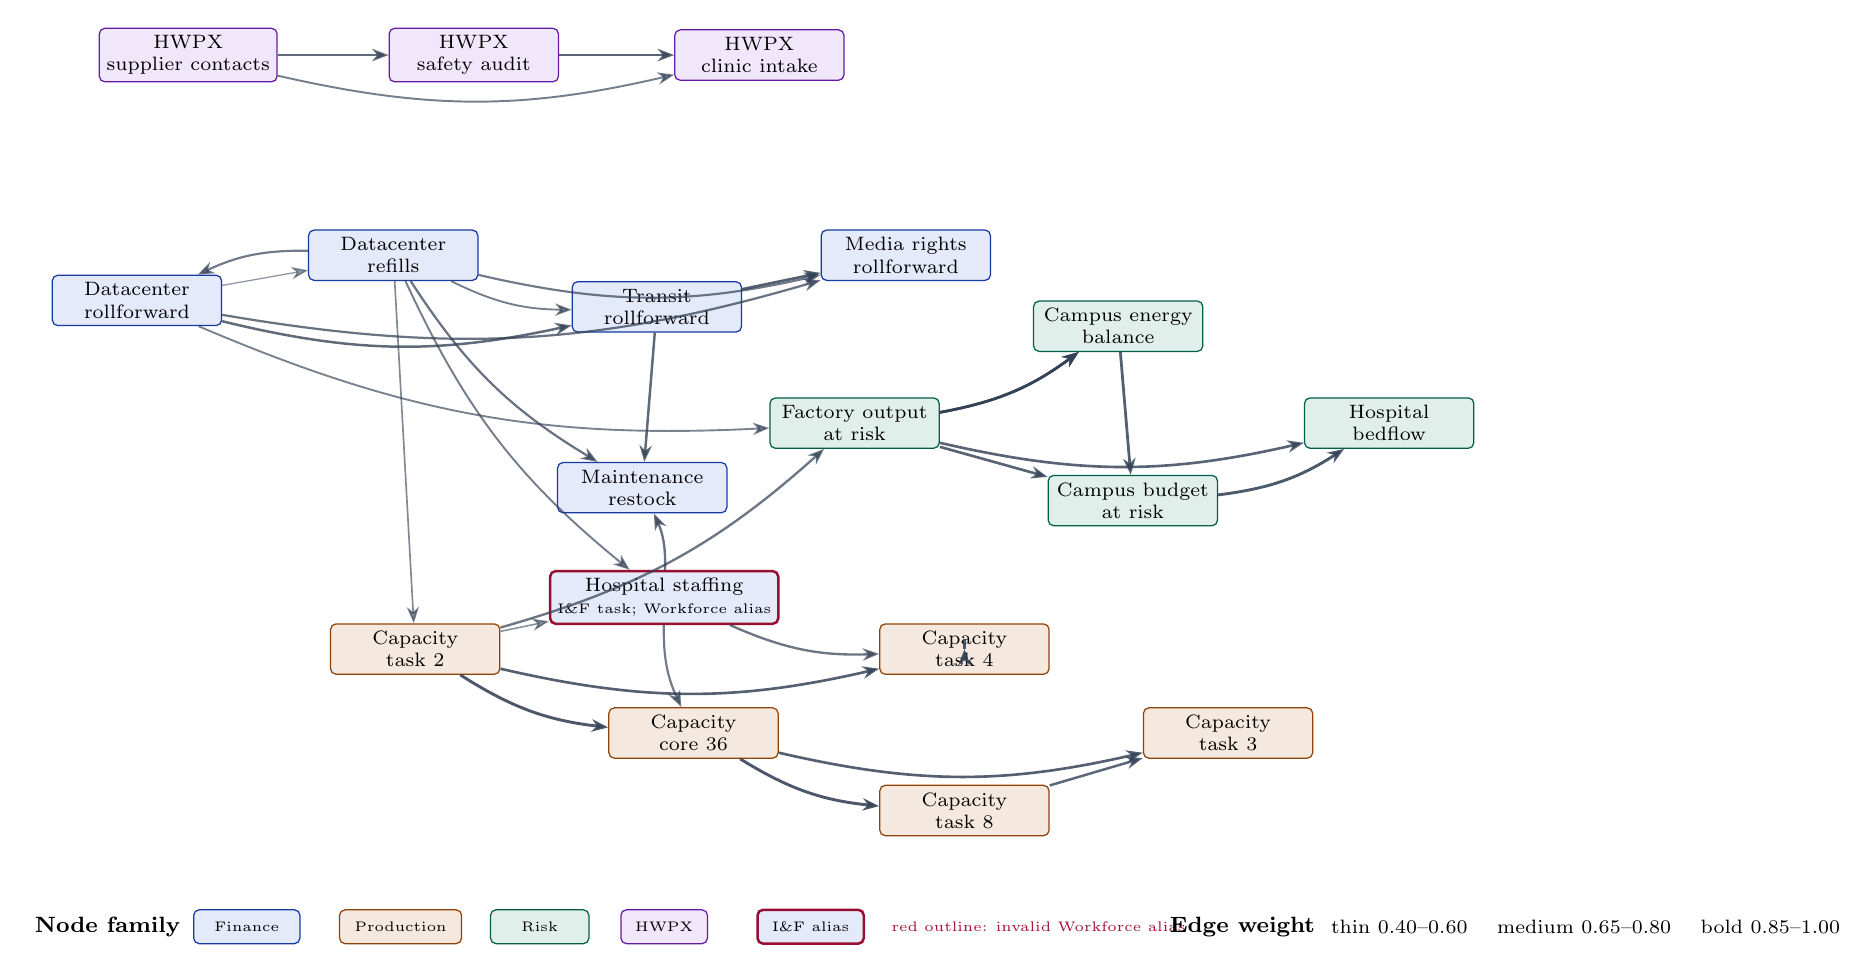
\begin{tikzpicture}[
  x=0.93cm,
  y=0.82cm,
  every node/.style={font=\scriptsize, align=center, inner sep=2.6pt},
  task/.style={draw, rounded corners=2pt, minimum width=2.15cm, minimum height=0.64cm, line width=0.45pt},
  financeNode/.style={task, fill=finance!12, draw=finance!75!black},
  productionNode/.style={task, fill=production!13, draw=production!80!black},
  riskNode/.style={task, fill=risk!12, draw=risk!80!black},
  hwpxNode/.style={task, fill=hwpx!11, draw=hwpx!80!black},
  anomalyNode/.style={task, fill=finance!12, draw=workforce!80!black, line width=0.9pt}
]
  % HWPX document-automation component.
  \node[hwpxNode] (supplier) at (-7.6, 5.1) {HWPX\\supplier contacts};
  \node[hwpxNode] (safety) at (-3.7, 5.1) {HWPX\\safety audit};
  \node[hwpxNode] (clinic) at (0.2, 5.1) {HWPX\\clinic intake};

  % Finance and integration component.
  \node[financeNode] (dc) at (-8.3, 1.3) {Datacenter\\rollforward};
  \node[financeNode] (refills) at (-4.8, 2.0) {Datacenter\\refills};
  \node[financeNode] (transit) at (-1.2, 1.2) {Transit\\rollforward};
  \node[financeNode] (maint) at (-1.4, -1.6) {Maintenance\\restock};
  \node[financeNode] (media) at (2.2, 2.0) {Media rights\\rollforward};

  % Production and workforce component.
  \node[productionNode] (p2) at (-4.5, -4.1) {Capacity\\task 2};
  \node[anomalyNode] (staffing) at (-1.1, -3.3) {Hospital staffing\\{\tiny I\&F task; Workforce alias}};
  \node[productionNode] (p36) at (-0.7, -5.4) {Capacity\\core 36};
  \node[productionNode] (p4) at (3.0, -4.1) {Capacity\\task 4};
  \node[productionNode] (p8) at (3.0, -6.6) {Capacity\\task 8};
  \node[productionNode] (p3) at (6.6, -5.4) {Capacity\\task 3};

  % Weighted-risk-assessment component.
  \node[riskNode] (factory) at (1.5, -0.6) {Factory output\\at risk};
  \node[riskNode] (energy) at (5.1, 0.9) {Campus energy\\balance};
  \node[riskNode] (budget) at (5.3, -1.8) {Campus budget\\at risk};
  \node[riskNode] (bedflow) at (8.8, -0.6) {Hospital\\bedflow};

  % HWPX edges: 0.70--0.90.
  \edgeS{supplier}{safety}{0.78}{0.85pt}
  \edgeR{supplier}{clinic}{0.68}{0.70pt}
  \edgeS{safety}{clinic}{0.82}{0.95pt}

  % Finance / production / workforce edges: 0.40--1.00.
  \edgeS{dc}{refills}{0.56}{0.45pt}
  \edgeR{dc}{transit}{0.78}{0.90pt}
  \edgeR{dc}{factory}{0.66}{0.68pt}
  \edgeR{dc}{media}{0.74}{0.80pt}
  \edgeR{refills}{dc}{0.70}{0.78pt}
  \edgeS{refills}{p2}{0.62}{0.60pt}
  \edgeR{refills}{staffing}{0.68}{0.70pt}
  \edgeR{refills}{transit}{0.68}{0.68pt}
  \edgeR{refills}{maint}{0.74}{0.80pt}
  \edgeR{refills}{media}{0.70}{0.78pt}
  \edgeS{p2}{staffing}{0.60}{0.55pt}
  \edgeR{p2}{factory}{0.72}{0.85pt}
  \edgeR{p2}{p4}{0.84}{0.95pt}
  \edgeR{p2}{p36}{0.88}{1.05pt}
  \edgeR{staffing}{maint}{0.74}{0.85pt}
  \edgeR{staffing}{p4}{0.72}{0.85pt}
  \edgeR{staffing}{p36}{0.70}{0.78pt}
  \edgeS{transit}{maint}{0.78}{0.90pt}
  \edgeS{transit}{media}{0.84}{0.95pt}
  \edgeR{p36}{p8}{0.88}{1.05pt}
  \edgeR{p36}{p3}{0.84}{0.95pt}
  \edgeR{p4}{p4}{0.88}{1.05pt}
  \edgeS{p8}{p3}{0.80}{0.90pt}

  % Weighted-risk-assessment edges. Parallel edges are intentionally retained.
  \edgeR{factory}{energy}{0.78}{0.90pt}
  \edgeR{factory}{energy}{0.82}{0.95pt}
  \edgeR{factory}{energy}{0.82}{0.95pt}
  \edgeS{factory}{budget}{0.82}{0.95pt}
  \edgeR{factory}{bedflow}{0.82}{0.95pt}
  \edgeS{energy}{budget}{0.84}{1.00pt}
  \edgeR{budget}{bedflow}{0.87}{1.05pt}

  % Legend.
  \node[anchor=west, font=\footnotesize\bfseries] at (-9.8, -8.4) {Node family};
  \node[financeNode, minimum width=1.35cm, minimum height=0.43cm, font=\tiny] at (-6.8, -8.4) {Finance};
  \node[productionNode, minimum width=1.55cm, minimum height=0.43cm, font=\tiny] at (-4.7, -8.4) {Production};
  \node[riskNode, minimum width=1.25cm, minimum height=0.43cm, font=\tiny] at (-2.8, -8.4) {Risk};
  \node[hwpxNode, minimum width=1.1cm, minimum height=0.43cm, font=\tiny] at (-1.1, -8.4) {HWPX};
  \node[anomalyNode, minimum width=1.35cm, minimum height=0.43cm, font=\tiny] at (0.9, -8.4) {I\&F alias};
  \node[anchor=west, text=workforce!85!black, font=\tiny] at (1.9, -8.4) {red outline: invalid Workforce alias};
  \node[anchor=west, font=\footnotesize\bfseries] at (5.7, -8.4) {Edge weight};
  \node[anchor=west, font=\scriptsize] at (7.9, -8.4) {thin 0.40--0.60 \quad medium 0.65--0.80 \quad bold 0.85--1.00};
\end{tikzpicture}
\end{center}

\vfill
\noindent\footnotesize
\textbf{Reading the figure.} The topology view coalesces parallel source-target records where they overplot. The following registry retains the full source, target, relation, and numeric weight for every one of the 38 directed edge records.

\newpage
\begin{center}
  {\Large\bfseries Edge Registry}\par
  \vspace{2pt}
  {\small Exact directed edge records in the batch-4 terminal snapshot}
\end{center}
\vspace{5pt}
\footnotesize
\renewcommand{\arraystretch}{1.12}
\begin{longtable}{@{}r >{\raggedright\arraybackslash}p{3.35cm} >{\raggedright\arraybackslash}p{3.35cm} >{\raggedright\arraybackslash}p{4.75cm} r@{}}
\toprule
\# & Source & Target & Relation & Weight \\
\midrule
\endfirsthead
\toprule
\# & Source & Target & Relation & Weight \\
\midrule
\endhead
1 & Datacenter rollforward & Datacenter refills & transfer logic and structure & 0.40 \\
2 & Datacenter refills & Capacity task 2 & transfer inventory rollforward logic & 0.55 \\
3 & HWPX supplier contacts & HWPX safety audit & transfer HWPX XML manipulation logic & 0.85 \\
4 & Datacenter refills & Hospital staffing & transfer capacity planning logic & 0.65 \\
5 & Capacity task 2 & Hospital staffing & transfer inventory replenishment logic & 0.50 \\
6 & Datacenter rollforward & Transit rollforward & transfer Excel reconciliation structure & 0.85 \\
7 & Datacenter refills & Transit rollforward & transfer rollforward logic & 0.60 \\
8 & Capacity task 2 & Factory output at risk & transfer production metrics logic & 0.75 \\
9 & Datacenter rollforward & Factory output at risk & transfer Excel formula mapping & 0.60 \\
10 & Factory output at risk & Campus energy balance & transfer advanced Excel formula mapping & 0.85 \\
11 & Factory output at risk & Campus energy balance & transfer weighted aggregation logic & 0.90 \\
12 & Campus energy balance & Campus budget at risk & transfer lookup and mapping logic & 0.95 \\
13 & Factory output at risk & Campus budget at risk & transfer statistical aggregation logic & 0.90 \\
14 & Campus budget at risk & Hospital bedflow & transfer identical spreadsheet workflow & 0.98 \\
15 & Factory output at risk & Hospital bedflow & transfer template formula mapping & 0.90 \\
16 & Datacenter refills & Maintenance restock & transfer inventory replenishment logic & 0.75 \\
17 & Transit rollforward & Maintenance restock & transfer Excel standard structure & 0.85 \\
18 & Factory output at risk & Campus energy balance & transfer Excel lookup and statistical logic & 0.90 \\
19 & Capacity task 2 & Factory output at risk & transfer production metric logic & 0.75 \\
20 & Datacenter refills & Transit rollforward & transfer financial rollforward logic & 0.70 \\
21 & Capacity task 2 & Capacity task 4 & transfer capacity schedule logic & 0.95 \\
22 & Hospital staffing & Capacity task 4 & transfer threshold detection logic & 0.75 \\
23 & Transit rollforward & Media rights rollforward & transfer Excel reconciliation structure & 0.95 \\
24 & Datacenter refills & Media rights rollforward & transfer ledgers reconciliation logic & 0.75 \\
25 & Capacity task 2 & Capacity core 36 & identical capacity planning logic & 1.00 \\
26 & Hospital staffing & Capacity core 36 & transfer threshold event tracking & 0.70 \\
27 & HWPX safety audit & HWPX clinic intake & transfer HWPX XML processing logic & 0.90 \\
28 & HWPX supplier contacts & HWPX clinic intake & transfer data normalization logic & 0.70 \\
29 & Hospital staffing & Maintenance restock & transfer inventory replenishment logic & 0.80 \\
30 & Datacenter refills & Maintenance restock & transfer replenishment scheduling logic & 0.75 \\
31 & Capacity core 36 & Capacity task 8 & identical capacity planning logic & 1.00 \\
32 & Hospital staffing & Capacity task 8 & transfer threshold event tracking & 0.70 \\
33 & Media rights rollforward & Datacenter rollforward & transfer Excel reconciliation structure & 0.95 \\
34 & Datacenter refills & Datacenter rollforward & transfer financial rollforward logic & 0.75 \\
35 & Datacenter rollforward & Media rights rollforward & transfer financial rollforward logic & 0.80 \\
36 & Capacity task 4 & Capacity task 4 & identical task specification & 1.00 \\
37 & Capacity core 36 & Capacity task 3 & identical capacity planning logic & 0.95 \\
38 & Capacity task 8 & Capacity task 3 & transfer capacity schedule logic & 0.90 \\
\bottomrule
\end{longtable}

\end{document}
